\chapter{Validation}
\label{sec:Validation}

This chapter is dedicated to the validation of the framework on real-world data. In \autoref{ch:FeatureExtraction}, the reference dataset \cite{lee2007bearingdataset} has been introduced. Firstly, the \texttt{\gls{glo:python}} implementation of the framework is validated on the \gls{ims} dataset several times with different configurations to show the flexibility of the framework, and try to find the best configuration for the dataset. 

The first test in the \gls{ims} dataset is carried out with all the implemented machine learning models, then only the K-mean model is used in the following tests. In all tests an outlier filter has been implemented, so that the \gls{mla} will warn about the novelty behaviour only if two consecutive \gls{glo:snap}s are labelled as outliers. The number of consecutive \gls{glo:snap}s is a parameter that can be adjusted in the framework settings.

Then, the \gls{glo:edge} implementation of the framework based on the K-means \gls{glo:clust}ing is validated experimentally on a machine and with a laboratory shaker.


\section{\gls{ims} dataset No.1 - Bearing 3x sensor}
\label{sec:ValidationOnRealWorldData}
\begin{figure}
    \centering
    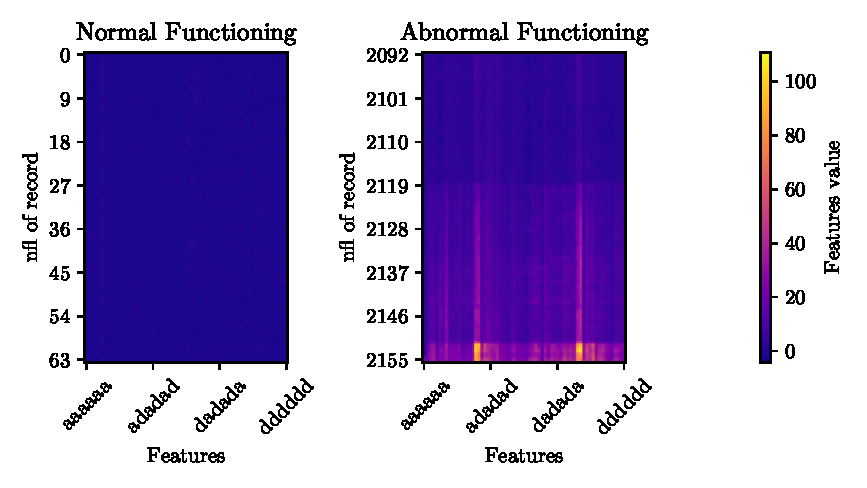
\includegraphics{images/IMS/Heatmap.pdf}
    \caption{Heatmap of the \gls{glo:std} features value for the test $\text{n}^\circ$1 of \gls{ims} dataset}
    \label{fig:Heatmap}
\end{figure}


To start the validation, the test No.1 of the \gls{ims} dataset is subdivided into \emph{training} and \emph{testing} datasets. The first 500 samples are used for training, and the remaining samples are used for testing. 

For all the algorithms, the assumption about the system is that, even if the degradation is continuous, the system is surely healthy until 2003-11-07. The threshold for performing the \gls{nd} is set conformingly to this assumption, for every model considered. Otherwise, the performance of any model could be artificially made as good as desired, by simply setting the threshold to a lower value.

The configuration file is set to use the data from the \quoted{bearing 3x} sensor, extracting all the time-domain and frequency-domain features described in \autoref{ch:FeatureExtraction}. The training dataset is used to train the \gls{mla} to recognize the normal behaviour of the bearing, and the testing dataset is used to validate the trained model. The \autoref{tab:IMS_test_parameters} shows the parameters of test No.1 of the \gls{ims} dataset. For display purposes, the features are \gls{glo:std}, and the heatmap of the \gls{glo:std} features is shown in \autoref{fig:Heatmap} in normal and abnormal conditions.

The abstract version of the \gls{fieldAg} has been used to extract the features from the dataset, creating all the \gls{glo:snap}s in the set $\gls{sym:snapset}=\{\gls{sym:snap}_1,\gls{sym:snap}_2,\dots,\gls{sym:snap}_{500}\}$. These \gls{glo:snap}s are stored in the \emph{unconsumed} collection of the database.

\subsection{Training - K-means}

Using the commands of the \gls{cli}, the training procedure has been launched:
\begin{minted}[linenos,breaklines]{bash}
    C:/Users/JohnSmith/Code/framework> python ./MASTER.py run-feature-agent
    C:/Users/JohnSmith/Code/framework> python ./MASTER.py run-machine-learning-agent novelty train
\end{minted}

where the first command runs the \gls{fieldAg} and the second one runs an \quoted{healthy} instance of the \gls{mla} in training mode.
At this point, the \gls{mla} asks the user to move the \gls{glo:snap}s from the \emph{unconsumed} to the \emph{healthy} collection, since the \emph{healthy} collection is empty. After the confirmation, the \gls{mla} starts the training with a different number of \gls{glo:clust}s and outputs the scoring in the form of silhouette and inertia scores. The results are shown in \autoref{fig:SilScore_01} and \autoref{fig:InertiaScore_01}. The user can confirm that the best number of \gls{glo:clust}s is 2, as the silhouette score is the highest and the inertia score is at the \gls{pof} point, or insert another number of \gls{glo:clust}s, remembering that it is best to overestimate the number of \gls{glo:clust}s to increase the system sensitivity, as discussed in \autoref{sec:wrong_k}. 

In this case, the number of \gls{glo:clust}s has been set to 2, so that the \gls{mla} saves the model trained with $n=2$ into the database. Even if the feature space has high dimensionality, the agent plot to the user also a scatter plot of a subset of features of the training dataset, to have a visual feedback of the \gls{glo:clust}ing, as shown in \autoref{fig:Clusters}, where the points are the \gls{glo:snap}s, the crosses are the centroids and the colours represent the assigned \gls{glo:clust}. We can observe that selecting 2 as the number of \gls{glo:clust}s is adequate and that the projections of the \gls{glo:clust}s' shapes on some planes are not perfectly spherical but, at least, they are not too elongated. This is a good sign for the K-means algorithm, as discussed in \autoref{sec:kmeans_limits}.

\begin{figure}
    \centering
    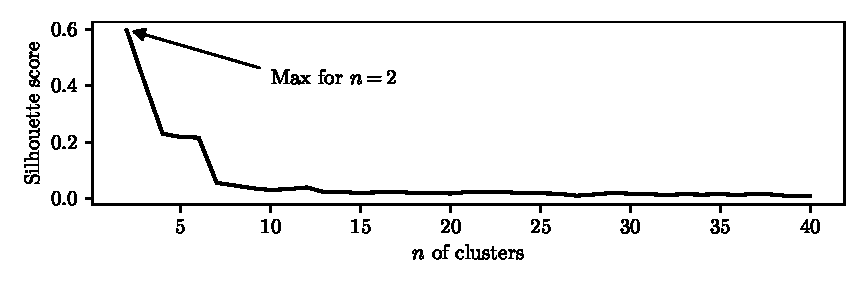
\includegraphics{images/IMS/SilScore_01.pdf}
    \caption{Silhouette score for \gls{glo:clust}ing the test $\text{n}^\circ$1 of \gls{ims} dataset (K-means)}
    \label{fig:SilScore_01}
\end{figure}

\begin{figure}
    \centering
    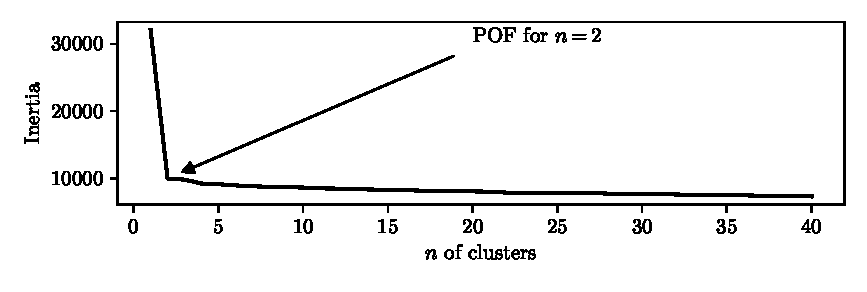
\includegraphics{images/IMS/InertiaScore_01.pdf}
    \caption{Inertia score for \gls{glo:clust}ing the test $\text{n}^\circ$1 of \gls{ims} dataset (K-means)}
    \label{fig:InertiaScore_01}
\end{figure}

\begin{figure}
    \centering
    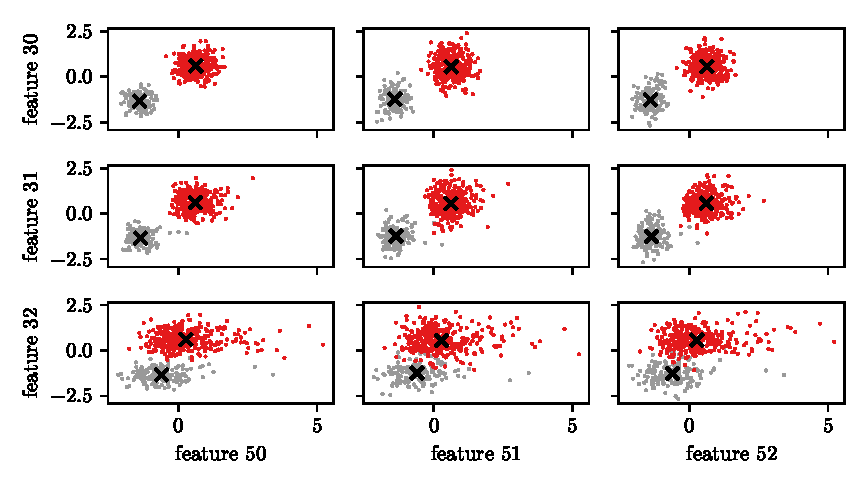
\includegraphics{images/IMS/Clusters.pdf}
    \caption{Scatterplot of training $\gls{glo:snap}$ for the test $\text{n}^\circ$1 of \gls{ims} dataset}
    \label{fig:Clusters}
\end{figure}

\subsection{\gls{nd} Validation - K-means}
Using the validation partition of the dataset, it is possible to set the \gls{mla} in \emph{evaluate} mode. The \gls{fieldAg} uses the validation partition and fills the \emph{raw} collection with the time-series. The {\gls{fa}} extract the features and continuously fill the \emph{unconsumed} collection with the \gls{glo:snap}s. The \gls{mla} evaluates the \gls{glo:snap}s according to \autoref{alg:eval_new_snapshot}  and plots the result, as well as generating a warning if the novelty metric is greater than a certain threshold (in this case 50\%, but it is configurable in the usual \texttt{.yaml} file). The results are shown in \autoref{fig:NoveltyScore_01}, where we can see that the framework detects the novelty quite early, at 2003-11-16 07:46, while the dataset authors, declared the test finished because of bearing defects (not catastrophic failures) at 2003-11-25 23:40. The comparison of the margin of early detection for different algorithms will be resumed later.

In \autoref{fig:NoveltyScore_01_detail}, a detailed view of the \gls{nd} metric becoming consistently greater than the threshold is shown.

\begin{figure}
    \centering
    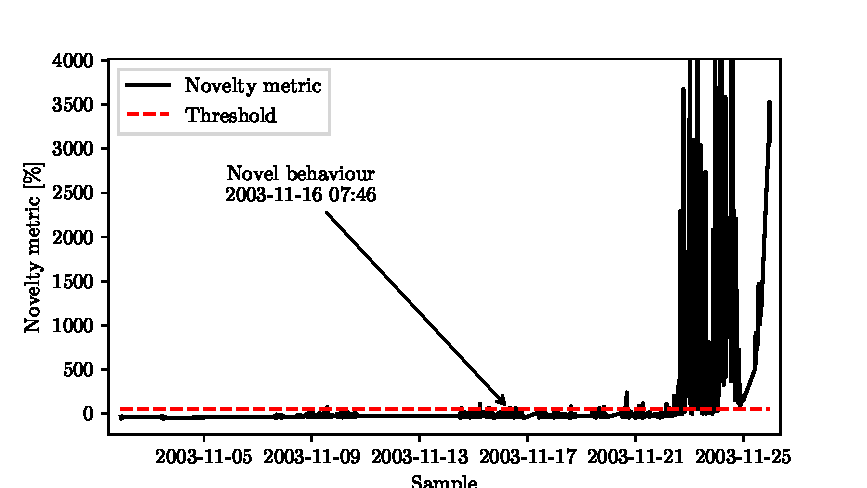
\includegraphics{images/IMS/Novelty_01_500samples_bearing3x.pdf}
    \caption{Results of \gls{nd} for the test $\text{n}^\circ$1 of \gls{ims} dataset (K-means)}
    \label{fig:NoveltyScore_01} 
\end{figure}

\begin{figure}
    \centering
    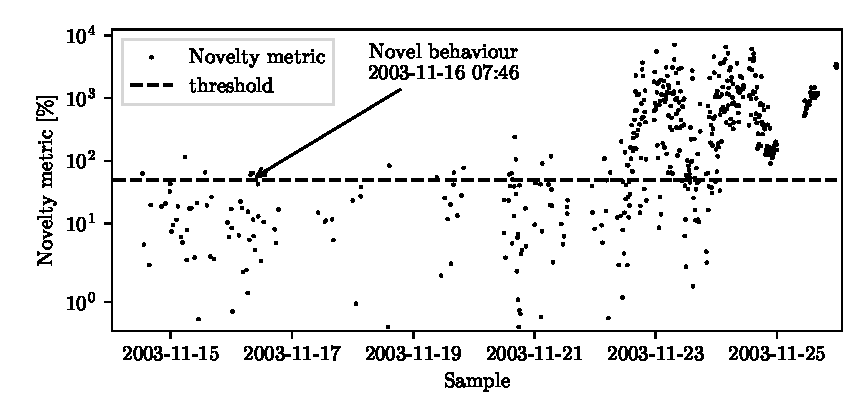
\includegraphics{images/IMS/Novelty_01_500samples_bearing3x_detail.pdf}
    \caption{Results of \gls{nd} for the test $\text{n}^\circ$1 of \gls{ims} dataset (K-means) - detailed view}
    \label{fig:NoveltyScore_01_detail} 
\end{figure}

\subsection{Training - \gls{dbscan}}
Using the same partition of the dataset as for the K-means training, we can train a \gls{dbscan} model. In this case, the silhouette score has to be used to select a suitable value of the radius $\varepsilon$. As shown in \autoref{fig:silscore_dbscan}, the optimal value is 8, which corresponds correctly to the generation of two \gls{glo:clust}s.

\begin{figure}
    \centering
    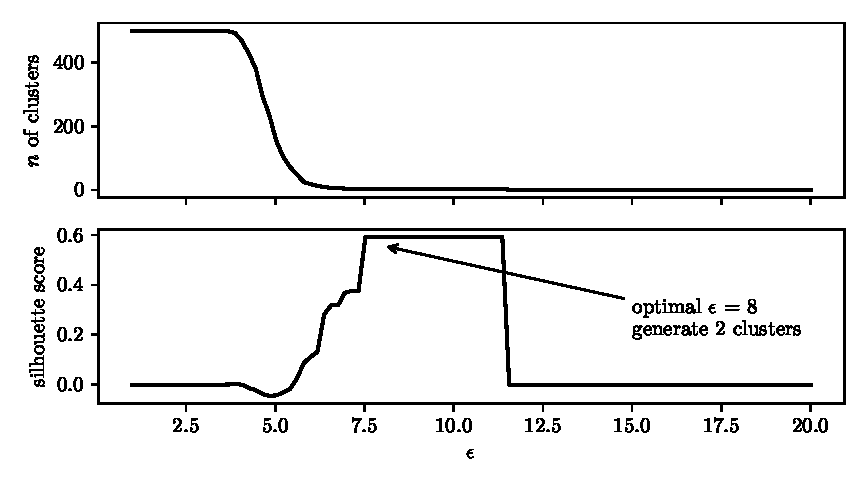
\includegraphics{images/IMS/InertiaScore_01_dbscan.pdf}
    \caption{Silhouette score for \gls{glo:clust}ing the test $\text{n}^\circ$1 of \gls{ims} dataset (\gls{dbscan})}
    \label{fig:silscore_dbscan}
\end{figure}

\subsection{\gls{nd} Validation - \gls{dbscan}}
As it has been done for the K-means, the validation partition of the dataset is now used for performing \gls{nd} with the \gls{dbscan} model, as described in \autoref{sec:dbscan_eval}. The result is shown in \autoref{fig:NoveltyScore_01_dbscan}, where we can see that the \gls{dbscan} model detects the novelty at 2003-11-22 15:06, that is quite early, but not as early as the K-means model. This is because the metric generated by the \gls{dbscan} model has a greater variance so, instead of increasing consistently, it overshoots the threshold quite before this time but fails to consistently stay above the threshold. 

\begin{figure}
    \centering
    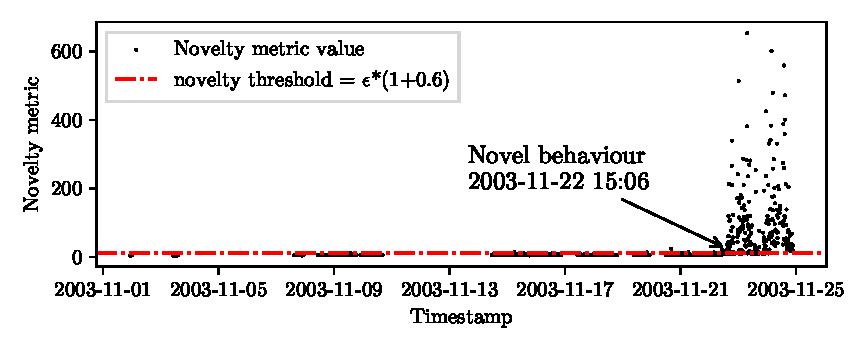
\includegraphics{images/IMS/Novelty_01_500samples_bearing3x_dbscan.pdf}
    \caption{Results of \gls{nd} for the test $\text{n}^\circ$1 of \gls{ims} dataset (\gls{dbscan})}
    \label{fig:NoveltyScore_01_dbscan}
\end{figure}

\subsection{Training - \gls{gmm}}
Let's now try with the \gls{gmm} model. The metric for selecting the number of \gls{glo:clust}s is now the \gls{bic} and the \gls{aic}, as shown in \autoref{fig:bic_aic_gmm}. The two metrics diverge but, as discussed in \autoref{sec:gauss_train}, the \gls{aic} tends to perform better. In this case, minimizing the \gls{aic} leads to select 25 as the number of \gls{glo:clust}s, which is much more than what was selected with the K-means, but still a reasonable choice, also considering that the \gls{gmm} is a soft \gls{glo:clust}ing algorithm and that we are using the density as a metric to perform \gls{nd}.

\begin{figure}
    \centering
    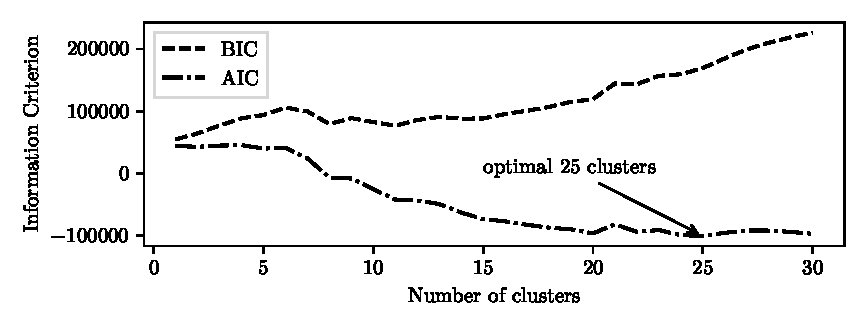
\includegraphics{images/IMS/BICAIC_GMM.pdf}
    \caption{\gls{bic} and \gls{aic} for \gls{glo:clust}ing the test $\text{n}^\circ$1 of \gls{ims} dataset (\gls{gmm})}
    \label{fig:bic_aic_gmm}
\end{figure}

\subsection{\gls{nd} Validation - \gls{gmm}}
The validation partition of the dataset is now used for performing \gls{nd} with the \gls{gmm} model. The result is shown in \autoref{fig:NoveltyScore_01_gmm}, where we can see that the \gls{gmm} model detects the novelty at 2003-11-22 03:47. The considerations about this result are the same as for the \gls{dbscan} model, and in fact, the timestamp of the detection event is really close to the one obtained with \gls{dbscan}. In \autoref{fig:NoveltyScore_01_gmm}, the metric (density value) appears in coloured dots, as each colour represents the \gls{glo:clust} to which the \gls{glo:snap} has been assigned.
\begin{figure}
    \centering
    \includegraphics{images/IMS/Novelty_01_500samples_bearing3x_gmm.pdf}
    \caption{Results of \gls{nd} for the test $\text{n}^\circ$1 of \gls{ims} dataset (\gls{gmm})}
    \label{fig:NoveltyScore_01_gmm}
\end{figure}

\subsection{\gls{nd} Validation - Bayesian \gls{gmm}}
The other Gaussian model is the \gls{bgmm}, since this approach is totally unsupervised, only the validation results are reported here. The result is shown in \autoref{fig:NoveltyScore_01_bgmm}, where we can see that the \gls{bgmm} model detects the novelty around the same time as the \gls{gmm} model, at 2003-11-22 03:45.

In both \gls{gmm} and \gls{bgmm} the metric (density value) spans a lot of decades, so the plots are done on a logarithmic scale.

\begin{figure}
    \centering
    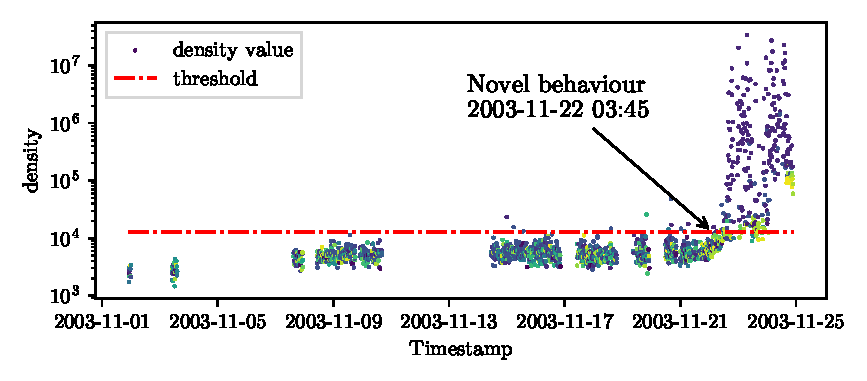
\includegraphics{images/IMS/Novelty_01_500samples_bearing3x_GMM_bayesan.pdf}
    \caption{Results of \gls{nd} for the test $\text{n}^\circ$1 of \gls{ims} dataset (\gls{bgmm})}
    \label{fig:NoveltyScore_01_bgmm}
\end{figure}

\subsection{\gls{nd} Validation - \gls{nu_svm}}
The next algorithm to test is the \gls{nu_svm}. Again, this is totally unsupervised, so only the validation results are reported here. The novelty metric evolution over time is shown in \autoref{fig:NoveltyScore_01_nusvm}, where we can see that the \gls{nu_svm} model detects the novelty at 2003-11-22 14:56, which is comparable with the \gls{dbscan} and \gls{gmm} models.

\begin{figure}
    \centering
    \includegraphics{images/IMS/Novelty_01_500samples_bearing3x_nusvm.pdf}
    \caption{Results of \gls{nd} for the test $\text{n}^\circ$1 of \gls{ims} dataset (\gls{nu_svm})}
    \label{fig:NoveltyScore_01_nusvm}
\end{figure}

\subsection{\gls{nd} Validation - \gls{iforest}}
The second last technique to test is the one based on the \gls{iforest} model. The result is shown in \autoref{fig:NoveltyScore_01_iforest}, where we can see that the \gls{iforest} model detects the novelty at 2003-11-16 10:08:46, which is a good result comparable with the K-means model. The problem with the metric of the \gls{iforest} is that it increases a lot the variance around the \gls{nd} event, but the mean does not increase consistently, so a lot of \gls{glo:snap}s are discarded as outliers, before the \gls{nd} event. 

This is, in my opinion, a promising approach. With these settings a lot of \gls{glo:snap}s are discarded as outliers, but with a different outlier filter, based on the percentage of novelty samples in a window, the \gls{iforest} model could perform even better.
\begin{figure}
    \centering
    \includegraphics{images/IMS/Novelty_01_500samples_bearing3x_iforest.pdf}
    \caption{Results of \gls{nd} for the test $\text{n}^\circ$1 of \gls{ims} dataset (\gls{iforest})}
    \label{fig:NoveltyScore_01_iforest}
\end{figure}

\subsection{\gls{nd} Validation - \gls{lof}}
The last algorithm to test is the \gls{lof}. The result is shown in \autoref{fig:NoveltyScore_01_lof}, where we can see that the \gls{lof} model detects the novelty at 2003-11-16 07:49, which is a good result comparable with the K-means model. It doesn't have the same problem as the \gls{iforest}, as there aren't as many discarded \gls{glo:snap}s before the \gls{nd} event.

\begin{figure}
    \centering
    \includegraphics{images/IMS/Novelty_01_500samples_bearing3x_lof.pdf}
    \caption{Results of \gls{nd} for the test $\text{n}^\circ$1 of \gls{ims} dataset (\gls{lof})}
    \label{fig:NoveltyScore_01_lof}
\end{figure}

\subsection{Comparison of the results}

\subsubsection{Comparison between the models}

\begin{table}
    \centering
    \caption{Comparison of the results for the test $\text{n}^\circ$1 of \gls{ims} dataset.}
    \label{tab:ims01_comparision}
    \begin{tabular}{lrr} 
    \toprule
    \textbf{Algorithm} & \textbf{\gls{nd} event} & \textbf{\gls{glo:leadtime} }{[}min] \\ 
    \hline
    K-means & 2003-11-16 07:46 & \textbf{13913} \\
    \gls{dbscan} & 2003-11-22 15:06 & 4833 \\
    \gls{gmm} & 2003-11-22 03:47 & 5513 \\
    \gls{bgmm} & 2003-11-22 03:45 & 5514 \\
    \gls{nu_svm} & 2003-11-22 14:56 & 4844 \\
    \gls{iforest} & 2003-11-16 10:08 & 13771 \\
    \gls{lof} & 2003-11-16 07:48 & 13912 \\
    {P2P} without any \gls{ml} & 2003-11-22 16:06 & 4774 \\
    \bottomrule
    \end{tabular}
\end{table}

In \autoref{tab:ims01_comparision}, the results of all the previous tests are resumed, together with the result of performing \gls{nd} without any machine learning algorithm, but just setting a threshold on the P2P value of the time-series, as it was previously shown in \autoref{fig:IMS_TD_features}. This last basic approach detects the novelty around the afternoon of 2003-11-22. 

The \gls{nu_svm} and the \gls{dbscan} models are not performing much better than not even using machine learning (at least on this dataset signal). The \gls{gmm} and \gls{bgmm} models are performing slightly better, but the margin is so low that the result may be biased by the threshold setting. The \gls{iforest}, \gls{lof} and K-means models are performing better, they are all very close to detecting the novelty, around 14000 min = 9.7 days before the end of the test. The K-means model is the one performing the best, but just slightly better than the \gls{iforest} and \gls{lof} models so, again, this small difference may not be significant. However, as discussed in the previous chapters, the K-means model will be used in the rest of the work, as it is also the most simple and interpretable model.


\subsubsection{Comparison with another approach}
As anticipated in the \autoref{ch:state_of_the_art}, about the State of the Art, the signal of the same bearing (Bearing 3x) of this same test has been used in \cite{Umberto}. In their research, the authors used a different approach, based on regression, and obtained the result reported in \autoref{fig:umbertoresult}


\subsubsection{Comment about the comparison}
Every system that outputs a warning based on a trigger on a threshold is highly sensitive to the value of the threshold itself. This means that the comparison of the results is not straightforward, and quite opinable, because selecting a low threshold will make almost every system trigger earlier. The measure to take into consideration, in my opinion, is how many false positives are generated if the threshold is lowered, and how small the variance of the metric is. A high variance, on this dataset, means that the system is very sensitive while evaluating quite similar signals.

\subsection{\gls{rul} Predictions validation - K-means}
After the \gls{nd} event, the \gls{mla} starts predicting the future evolution of the novelty metric, and it superimposes the prediction curve to the same plot displayed to the user. The fitting procedure is the closed form solution of the \gls{ls} problem applied to an exponential curve of \autoref{eq:exp_degradation_2}, as described in \autoref{sec:predictions}. The samples used for the regression of the curve are the last 230 before the current one. This parameter of the framework is configurable in the \texttt{.yaml} file. 

Some good predictions are shown in \autoref{fig:RULPredictions01}. The \gls{rul} is the difference between the intercept of the prediction curve and another threshold, higher than the one used for \gls{nd}, and the current time. In the figure, the blue line is a prediction made just a few hours after the \gls{nd} event (the vertical dashed line marks the time of the prediction). The same concept applies to the other predictions performed in later times.

In some circumstances, the novelty metric starts decreasing slightly, on average, as can be seen around 2003-11-21. In this case, if the novelty metric has this behaviour for several \gls{glo:snap}s ($\approx 230$), the fitted curve will be a decreasing exponential, as shown in \autoref{fig:RULPredictions01_fail}. 

If this situation occurs, the intercept with the threshold does not exist, and the \gls{rul} prediction fails, so the interpretation of the \gls{rul} is left to the user. In some cases, the defect in a system can \quoted{self-heal} (for example a crack in a bearing can be polished with the use \cite{IMSpaper}). If this behaviour is possible for the system, this situation can be interpreted as a sign that the system is going to return to normality. Otherwise, the user can retain the previous \gls{rul} prediction as the \gls{rul} of the system.

\begin{figure}
    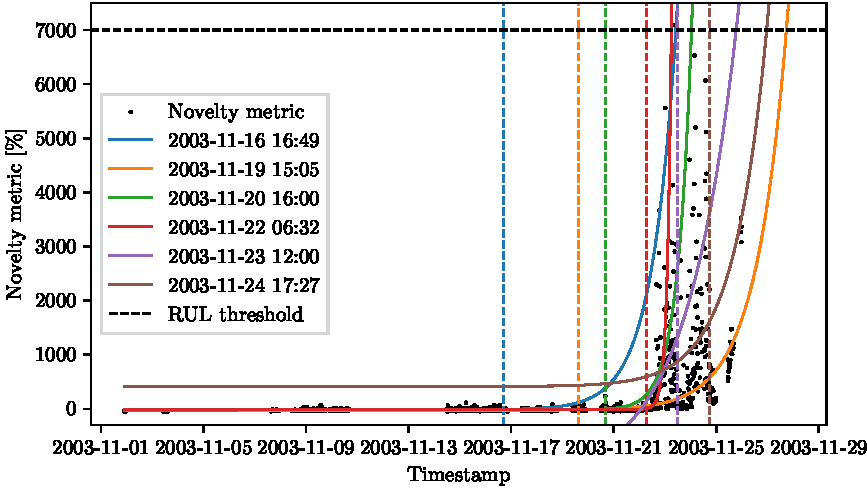
\includegraphics{images/IMS/Novelty_01_500samples_bearing3x_predictions.pdf}
    \caption{\gls{rul} prediction at different instants after the \gls{nd} event (dashed lines are the instants of the predictions corresponding to the same-colour solid line prediction)}
    \label{fig:RULPredictions01}
\end{figure}

\begin{figure}
    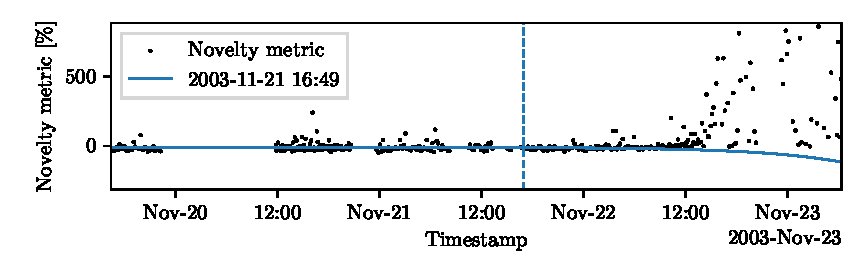
\includegraphics{images/IMS/Novelty_01_500samples_bearing3x_predictions_failed.pdf}
    \caption{Failed \gls{rul} prediction.}
    \label{fig:RULPredictions01_fail}
\end{figure}

\subsection{Retraining,  evaluating and predicting after \gls{nd} event}
If the user, after the \gls{nd} event, performs an investigation that leads to the belief that the system is still healthy, the user can turn the \gls{mla} in \emph{retrain} mode. In this case, the \gls{glo:snap}s that are in the quarantine collection, are moved to the healthy collection (faulty if the instance is for \gls{fd} and the investigation reveals that the fault is real). 
The model is then retrained with the new data with the same procedure used for the first training (silhouette and inertia scores are computed and the user is asked to confirm the number of \gls{glo:clust}s).

Let's investigate what would have happened if the user declared the system healthy at 2003-11-23 00:00, in the previous scenario of  \quoted{Bearing 3 x} signal in the \gls{ims} dataset. The \gls{mla} suggests that the best number of \gls{glo:clust}s is still two, so it has been retrained with the new data. The result of the updated model performing \gls{nd} is shown in \autoref{fig:NoveltyScore_01_retrained}. The predictions of the \gls{rul} are shown in \autoref{fig:RULPredictions01_retrained}. 

This test shows that in an increasingly decaying system retrained with data very close to the fault condition the \gls{mla} is able to detect the fault again. This comes at the cost of a later detection, and the first predictions after the \gls{nd} event are not as good as the previous ones. Anyway, the \gls{rul} predictions still become more accurate as time passes, and the \gls{rul} prediction at the end of the test is still quite accurate (on the same day of the event). 

Another consideration is about the \gls{rul} threshold: since the model has been retrained with \quoted{worse} data, the threshold for the \gls{rul} prediction should be set to a lower value, because now the \gls{glo:clust}s are either more in quantity, distorted or bigger, so it is unlikely that the novelty metric can still reach the same high values estimated before the retraining.

An intuition about why the sensitivity of the system is reduced after the retraining comes by examining the scatter plot of the \gls{glo:snap}s in the feature space, shown in \autoref{fig:Clusters_novelty}, where all the \gls{glo:snap}s extracted from the dataset are displayed. The \gls{glo:clust}s are more elongated and much bigger. These shapes arise gradually from the original ones of \autoref{fig:Clusters} so, by performing a retrain, both the effect of producing bigger \gls{glo:clust}s and one of the \gls{glo:clust}s being much more elongated play a role in reducing the sensitivity of the \gls{mla}.

\begin{figure}
    \centering
    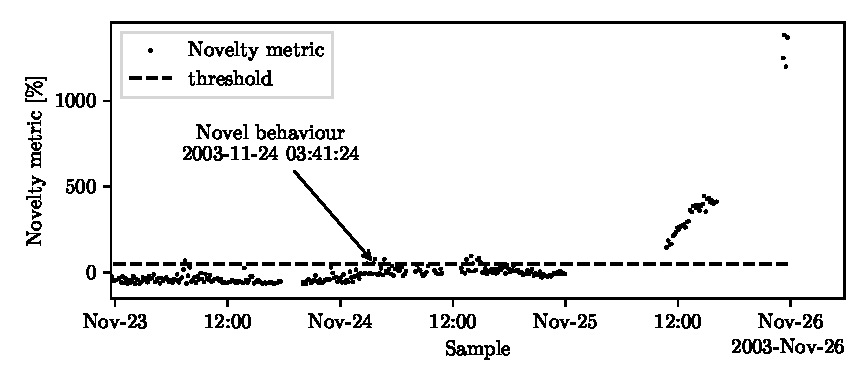
\includegraphics{images/IMS/Novelty_01_500samples_bearing3x_retrained.pdf}
    \caption{Results of \gls{nd} for the test $\text{n}^\circ$1 of \gls{ims} dataset (K-means) - retrained model}
    \label{fig:NoveltyScore_01_retrained}
\end{figure}

\begin{figure}
    \centering
    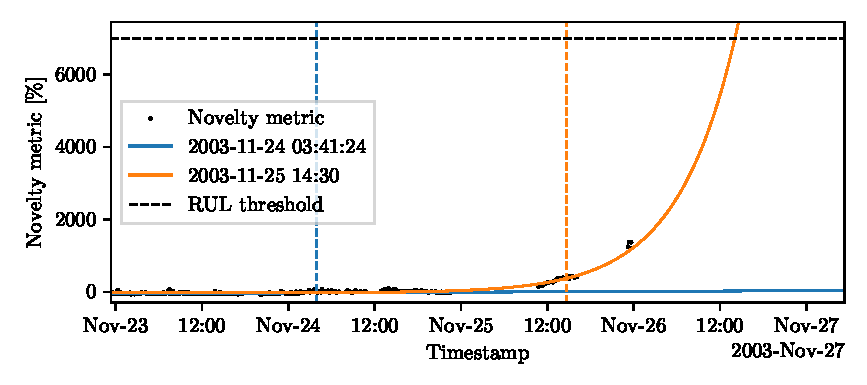
\includegraphics{images/IMS/Novelty_01_500samples_bearing3x_predictions_retrained.pdf}
    \caption{\gls{rul} prediction at different instants after the \gls{nd} event with the retrained model (dashed lines are the instants of the predictions corresponding to the same-colour solid line prediction)}
    \label{fig:RULPredictions01_retrained}
\end{figure}

\begin{figure}
    \centering
    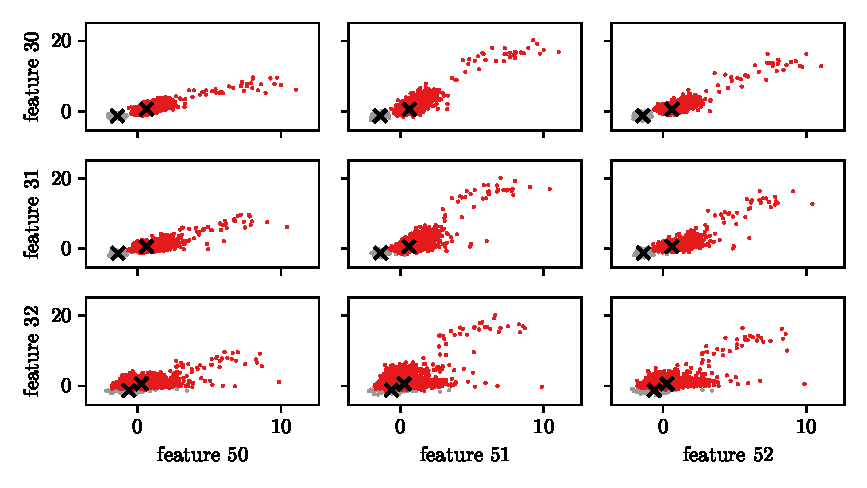
\includegraphics{images/IMS/Clusters_novelty.pdf}
    \caption{Scatterplot of all the $\gls{glo:snap}$ for the test $\text{n}^\circ$1 of \gls{ims} dataset}
    \label{fig:Clusters_novelty}
\end{figure}


\section{\gls{ims} dataset No.1 - All sensors}
In the previous section, an extensive test of the framework has been performed on a single signal from the dataset (Bearing 3 x). So the warning given by the \gls{mla} was indicating a problem in a specific component of the maintained system. Let's now test a configuration that takes in account all the signals of the dataset, so all the eight signals from the four bearings are used for feature extraction. This configuration should be able to detect a generic novel behaviout of the system or, better, a situaton in wich the sistem is abnormal as a whole (the signals may be normal but the combination of them may be abnormal).  In this case the configuration file has been set to use all the time-domain and all the frequency-domain features, and the \gls{mla} has been trained with the same procedure as before. 
\todo
\section{\gls{ims} dataset No.2 - Bearing 3x sensor}
\label{sec:IMS_n2_3x}

In the previous sections, the framework capability on detecting novelties has been tested. Looking back to the \autoref{tab:IMS_test_parameters}, the dataset No.2 share the same type of fault as the dataset No.3.

In order to further validate the \gls{nd}, in this section, a fresh training on the dataset no.2 is performed. This time using the \gls{mla} for both performing the \gls{nd} and \gls{fd}.

\subsection{\gls{nd} instance}
The first instance of the \gls{mla} is used to detect the \gls{nd} event. The sensor declared in the configuration file is the one of Bearing 1, because it is the one that will experience outer race failure. The training is done on the first 300 snapshots of the dataset. The silhouette criterion suggested to use 2 clusters. The \gls{mla} is then switched in evaluation mode, as usual. The novelty metric computed for the rest of the dataset is shown in \autoref{fig:IMS_n2_3x_nd}. 

The \gls{nd} event is triggered at 2004-02-16 03:32, 3~days before the end of the data acquisition. After the event, the novelty metric stays consistently over the threshold. 

\begin{figure}
    \centering
    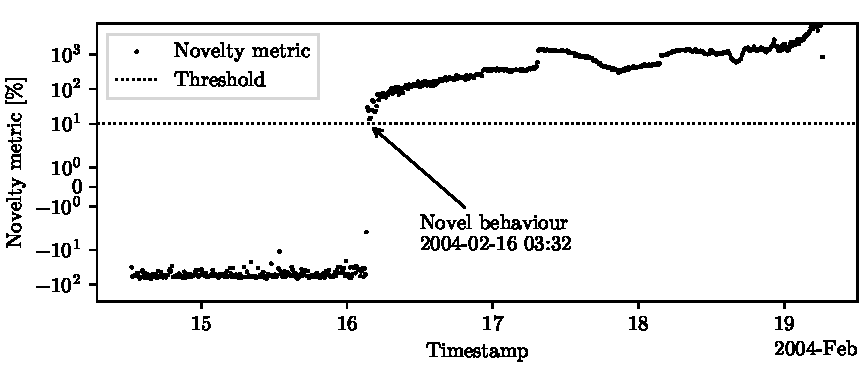
\includegraphics{images/IMS/Test02/ND.pdf}
    \caption{Novelty detection on the \gls{ims} dataset No.2 using the sensor of Bearing 1}
    \label{fig:IMS_n2_3x_nd}
\end{figure}

At this point, the \gls{rul} can be predicted at various instants after the \gls{nd} event. The \gls{rul} predictions are shown in \autoref{fig:IMS_n2_3x_prediction}. The predictions are made consigering the last 250 snapshots of the dataset. Most predictions are accurate, except for the one done at 2004-02-18 03:32, that is effected by the temporary local decrease of the novelty metric. In this case, the last \gls{rul} estimation should be retained.

\begin{figure}
    \centering
    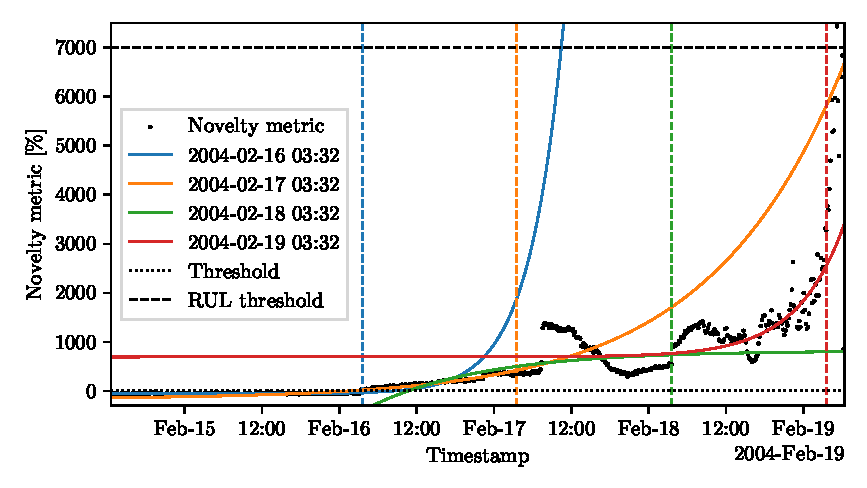
\includegraphics[width=\textwidth]{images/IMS/Test02/RUL.pdf}
    \caption{\gls{rul} prediction at different instants after the \gls{nd} event (dashed lines are the instants of the predictions corresponding to the same-colour solid line prediction)}
    \label{fig:IMS_n2_3x_prediction}
\end{figure}

\subsection{\gls{fd} instance}
The second instance of the \gls{mla} is used to detect the \gls{fd} event. The last 75 snapshots of the dataset are used for training. The silhouette criterion suggested to use 8 clusters. The \gls{mla} is then switched in evaluation mode. 

In this case, hte novelty metric provided by the \gls{mla} will be the transformed version, according with \autoref{eq:clust_eval_log}. In this case, a positive value of the metric coresponds to a known fault. When the metric becomes positive, the snapshot is already inside a faulty cluster, so the \gls{fd} event is triggered using a negative threshold. The novelty metric computed for the rest of the remaining samples in the dataset, after the set used to train the \emph{healthy} model and before the set used to train the \emph{faulty} model. The resulting metric is shown in \autoref{fig:IMS_n2_3x_fd}.

The \gls{fd} event is triggered at 2004-02-18 03:32, 1~day after the \gls{nd} event. After the event, the last 250 values of the novelty metric are used for \gls{rul} prediction. 

This example illustrate a scenario in wich the \gls{nd} event is detected firstly, and then the \gls{fd} event confirms the presence of a known fault in the system.

\begin{figure}
    \centering
    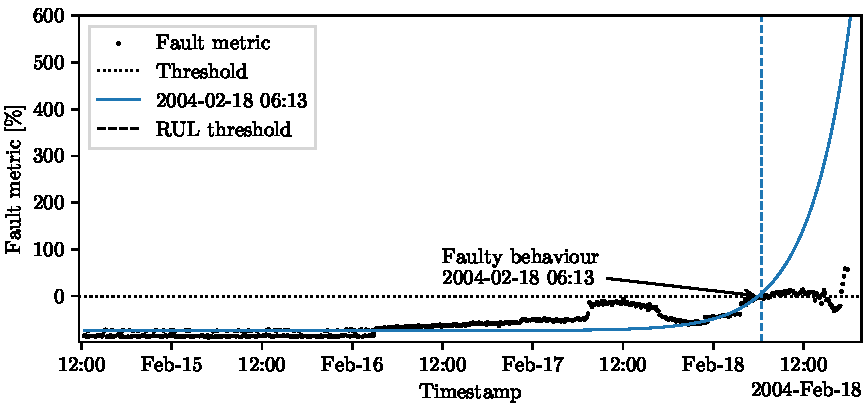
\includegraphics{images/IMS/Test02/FD.pdf}
    \caption{Fault detection on the \gls{ims} dataset No.2 using the sensor of Bearing~1}
    \label{fig:IMS_n2_3x_fd}
\end{figure}

\todo
\section{\gls{ims} dataset No.3 - Bearing 3 sensor}
\label{sec:IMS_n3_3x}

\subsection{\gls{nd} instance}

In the previous section about the \gls{ims} dataset No.2, the \gls{glo:frmwrk} capability for detecting novelties and known faults has been tested. The third dataset exploits the same fault as the second dataset. This enables testing the \gls{glo:frmwrk} capability on detecting novelties and known faults on a new bearing, without retraining the model from scratch. In this case, the outer race failure is experienced by Bearing 3, so the sensor declared in the configuration file is the one for this bearing.

Running the \gls{mla} in evaluation mode, the novelty metric computed for the first 300 \gls{glo:snap}s of the dataset, is shown in \autoref{fig:IMS_n3_3x_nd}. All the \gls{glo:snap}s are considered novelties. This means that the new bearing behaves differently from the previous ones. 

\begin{figure}
    \centering
    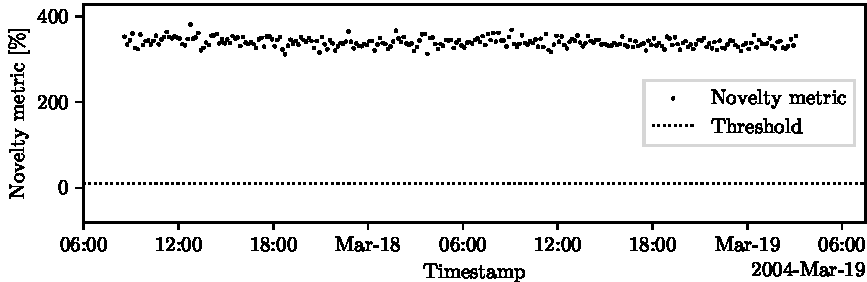
\includegraphics{images/IMS/Test03/retrain.pdf}
    \caption{Novelty detection on the \gls{ims} dataset No.3 using the sensor of Bearing 3, and the previous model trained on the dataset No.2}
    \label{fig:IMS_n3_3x_nd}
\end{figure}

The \gls{mla} saved all these \gls{glo:snap}s in the \emph{quarantined} collection. At this point, the \gls{mla} is switched to re-training mode, and the \emph{quarantined} collection is used to update the model. The silhouette criterion suggested using 2 \gls{glo:clust}s. Since the previous model was already trained with two \gls{glo:clust}s, this means that the new training data are assigned to existing \gls{glo:clust}s, enlarging them, instead of generating a new \gls{glo:clust}. 

The updated model is then switched to evaluation mode. The novelty metric computed for the rest of the dataset is shown in \autoref{fig:IMS_n3_3x_nd_updated}. The \gls{nd} event is triggered at 2004-04-12 19:21, $\approx$ 5~days before the end of the data acquisition. After the event, the novelty metric returns to the same level as before the event for two more days, before increasing again over the threshold and remaining consistently over the threshold.

\begin{figure}
    \centering
    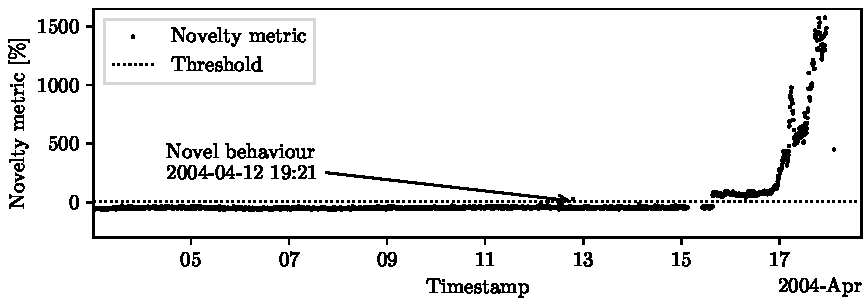
\includegraphics[width=\textwidth]{images/IMS/Test03/ND.pdf}
    \caption{Novelty detection on the \gls{ims} dataset No.3 using the sensor of Bearing 3, and the previous model updated}
    \label{fig:IMS_n3_3x_nd_updated}
\end{figure}

At this point, the \gls{rul} can be predicted. The predictions made considering the last 250~\gls{glo:snap}s of the dataset are shown in \autoref{fig:IMS_n3_3x_prediction}. The first prediction shown is made at the same time as the \gls{nd} event. Even with only two \gls{glo:snap}s exceeding the threshold, the fitted curve is correctly diverging. This first \gls{rul} prediction is quite accurate. The second fit in the figure is made when the novelty metric started to increase abruptly, so it results in a very short \gls{rul} prediction, shorter than the actual remaining time of the dataset.

\begin{figure}
    \centering
    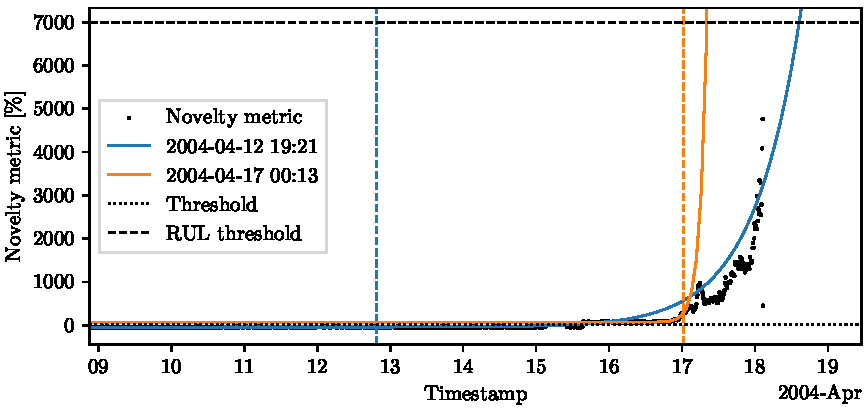
\includegraphics[width=\textwidth]{images/IMS/Test03/RUL.pdf}
    \caption{\gls{rul} prediction at different instants after the \gls{nd} event (dashed lines are the instants of the predictions corresponding to the same-colour solid line prediction)}
    \label{fig:IMS_n3_3x_prediction}
\end{figure}

\subsection{\gls{fd} instance}

The same test done for the \gls{nd} instance, can be repeated for the \gls{fd} instance of the \gls{mla}. The threshold is the same as for the previous test on dataset No. 2. The \gls{glo:frmwrk} is set in fault evaluation mode, and all the dataset is analyzed. 

The fault score evolution over time is shown in \autoref{fig:IMS_n3_3x_fd}. 
The \gls{fd} event is triggered at 2004-04-17 17:33, hours before the fault.
An increasing pattern appears quite before the \gls{fd} event, and before that, the metric is very steady. This allows lowering the threshold to trigger the \gls{fd} event earlier.

Another observation about the fault metric is that, even at its maximum value, it remains still negative. This means that the pattern in the \gls{glo:feature} space becomes closer and closer to the fault \gls{glo:clust}, as time passes, without actually entering the \gls{glo:clust} boundaries.

\begin{figure}
    \centering
    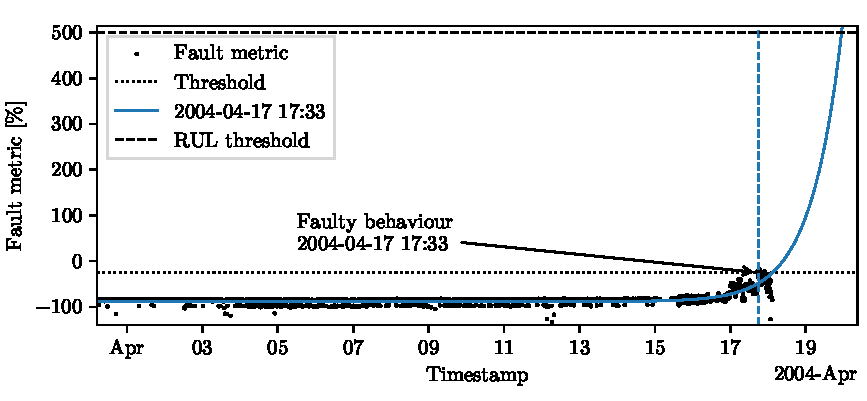
\includegraphics{images/IMS/Test03/FD.pdf}
    \caption{Fault detection on the \gls{ims} dataset No.3 using the sensor of Bearing 3}
    \label{fig:IMS_n3_3x_fd}
\end{figure}
\section{Experiments on a laboratory shaker - Test 1}
\label{sec:shaker_test01}

After the \gls{pc} implementation of the \gls{glo:frmwrk} has been tested widely on the \gls{ims} dataset, the \gls{glo:edge} implementation had to be validated experimentally. The first test was done with a laboratory shaker, which is basically a powerful active speaker with a really wide band that can be attached with a bolt to a structure, to vibrate it.

In this case, an accelerometer, whose key specifications are shown in \autoref{tab:adxl335_specifications}, was used to capture the vibration signal. The accelerometer was attached to the shaker, with a custom 3D-printed fixture. This first test has the scope of checking the capability of the \gls{glo:edge} implementation to detect a new low amplitude harmonic in the signal. The signal is generated as a \texttt{.wav} file and fed to the shaker by a player. Both the input of the shaker and the output of the accelerometer were monitored with a digital oscilloscope. The setup is shown in \autoref{fig:shaker_setup}.



\begin{table}[h]
    \centering
    \caption{Specifications of the ADXL335 Accelerometer}
    \label{tab:adxl335_specifications}
    \begin{tabular}{ll} 
    \toprule
    \textbf{Parameter} & \textbf{Value} \\ 
    \hline
    Supply Voltage & 1.8V to 3.6V \\
    Sensing Range & ±3g \\
    Sensitivity & 300 mV/g \\
    Bandwidth & 0.5 Hz to 1600 Hz \\
    Output Type & Analog \\
    Output Voltage Range & 0V to V$_{CC}$ \\
    Operating Temperature & -40°C to +85°C \\
    Package & $3\si{mm} \times 5 \si{mm} \times 1 \si{mm}$ \\
    \bottomrule
    \end{tabular}
\end{table}

\begin{figure}
    \centering
    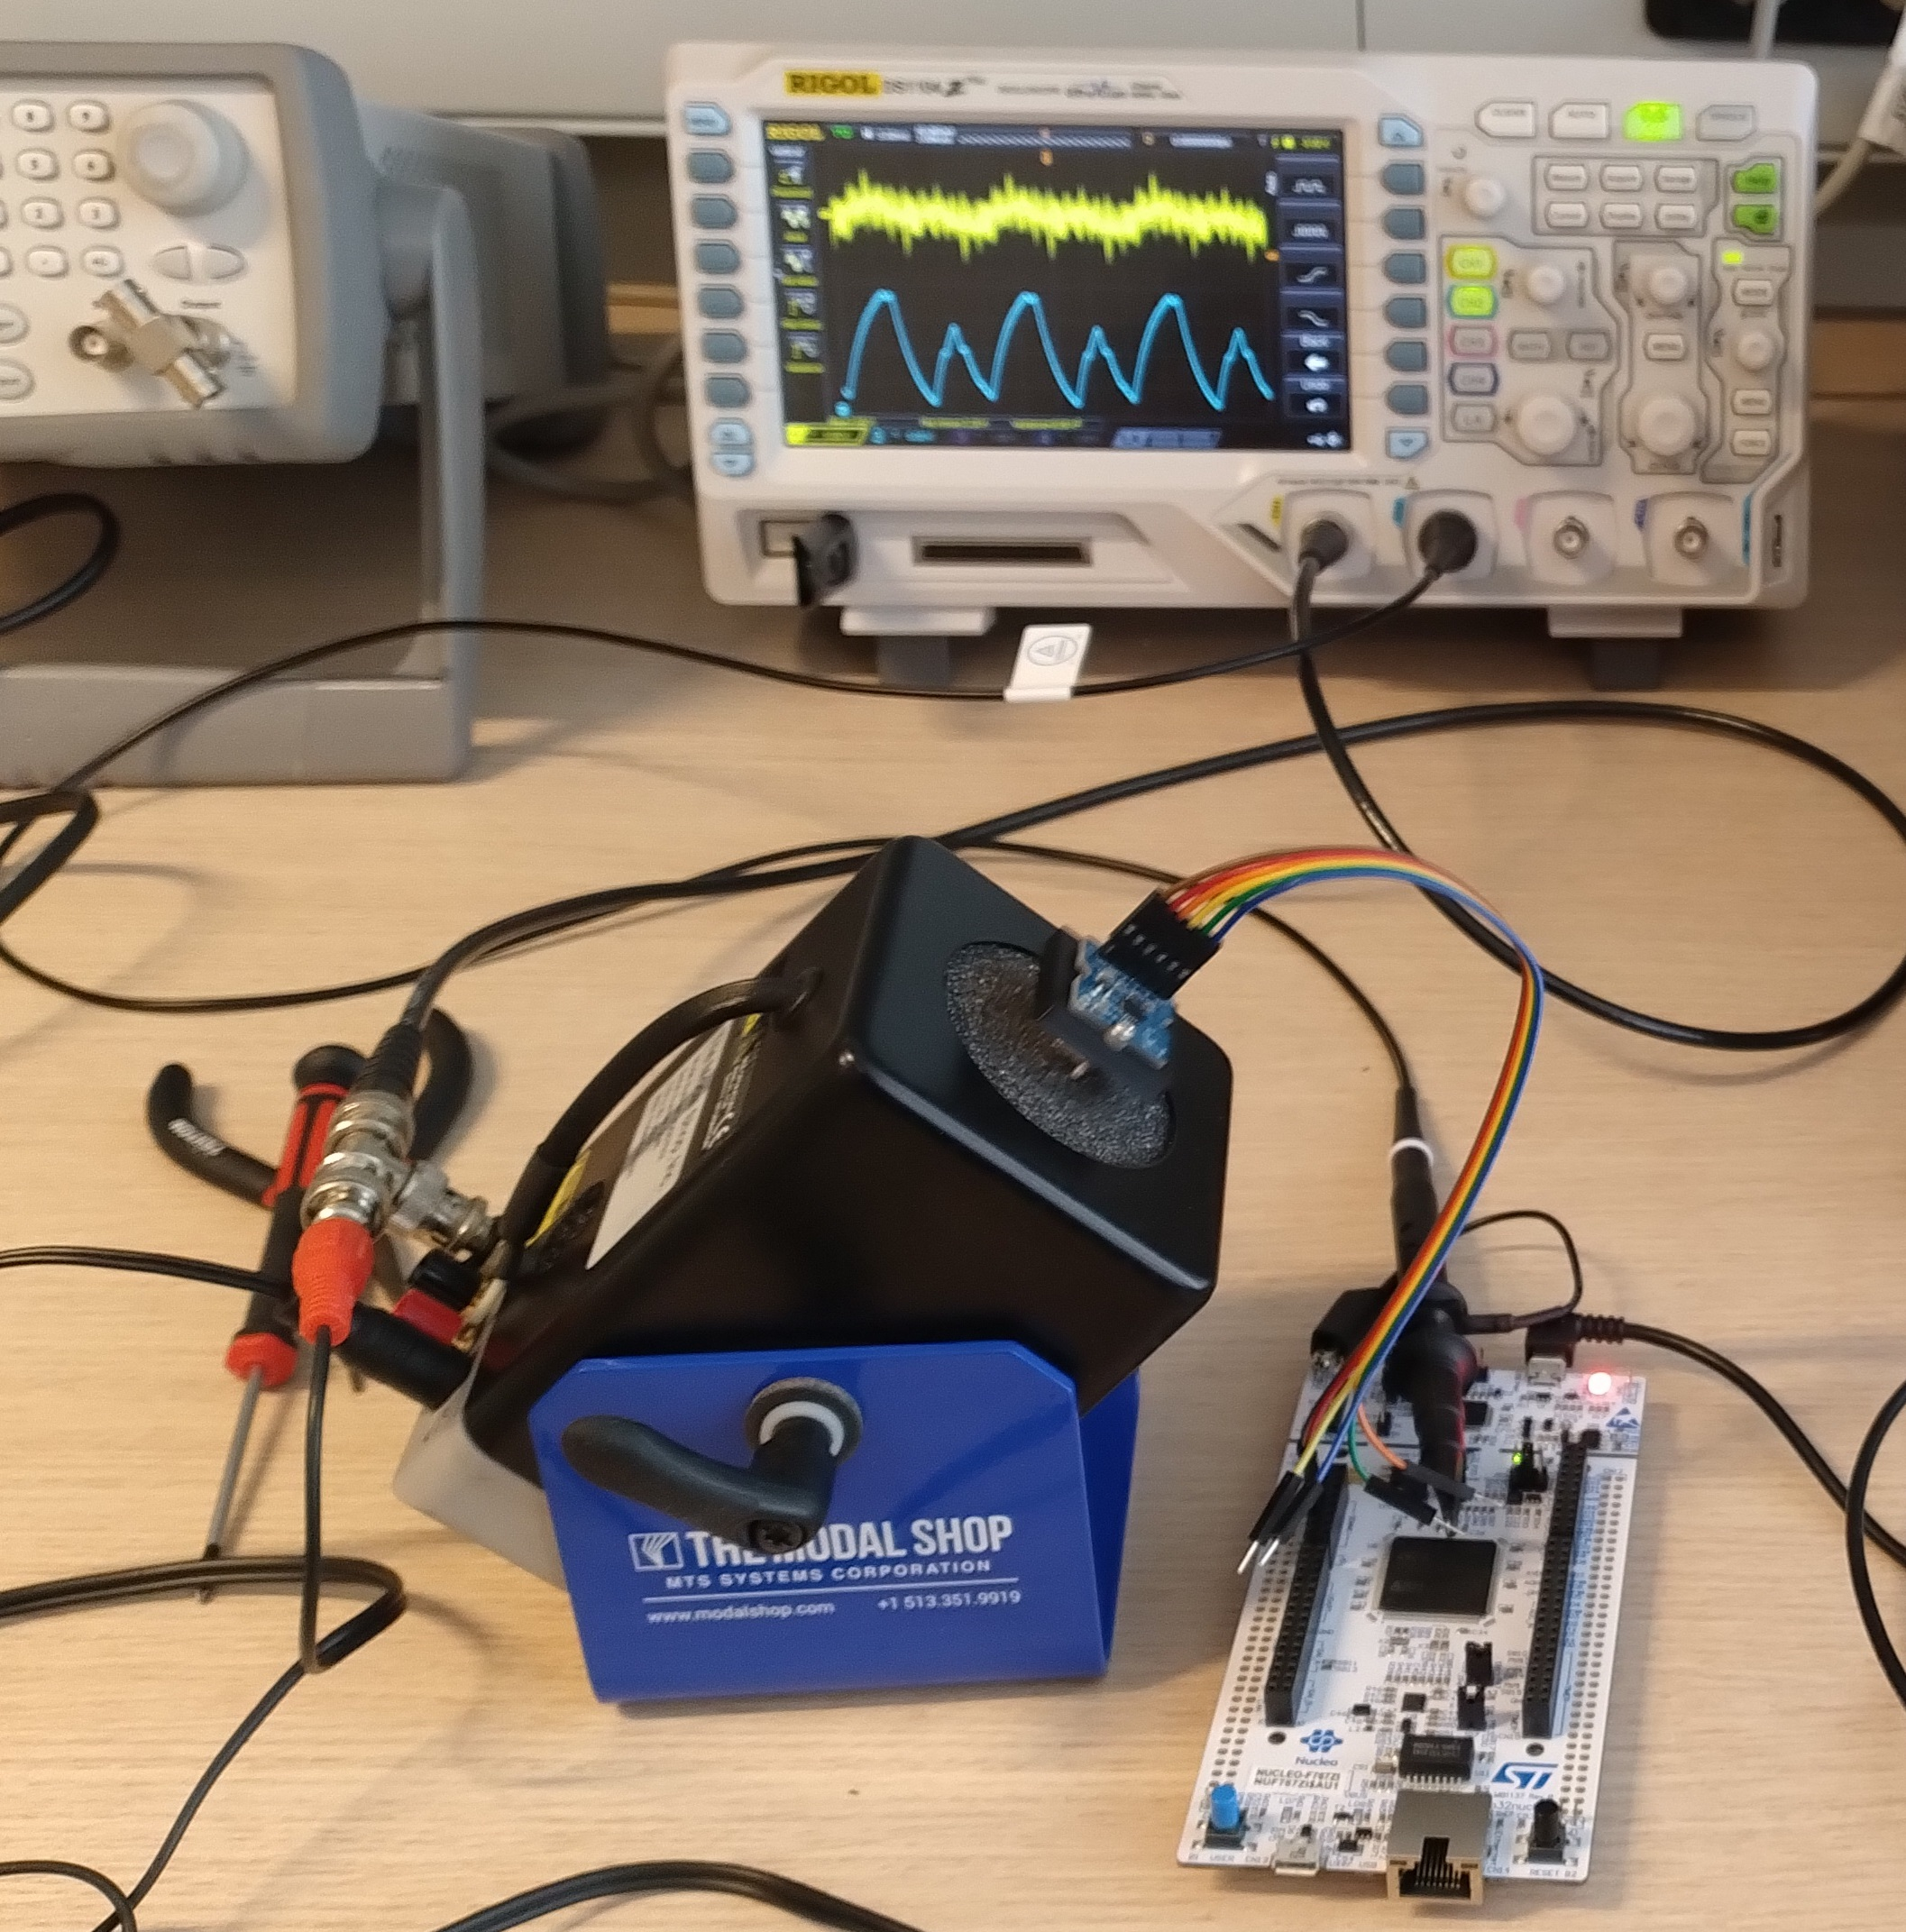
\includegraphics[width=.4\textwidth]{Images/shaker/IMG_20231207_103126143.jpg}
    \caption{Setup of the shaker tests.}
    \label{fig:shaker_setup}
\end{figure}
\begin{table}
    \centering
    \caption{Harmonic coefficients for the shaker test. Wave 1 and Wave 2 are training signals, and Harmonic Injection is the signal to be detected.}
    \label{tab:shaker_param_01}
    \begin{tabular}{lccccccc} 
    \toprule
    \multirow{2}{*}{\textbf{Signal Name }} & \multicolumn{6}{c}{\textbf{Harmonic frequency} [Hz]} & \multirow{2}{*}{\textbf{Amplitude} [mV]$_{pp}$} \\
     & 30 & 70 & 100 & 300 & 800 & 1400 &  \\ 
    \hline
    Wave 1 & 0.1 & 1.0 & 1.0 & \multicolumn{1}{c}{-} & 1.0 & 1.0 & 1000 \\
    Wave 2 & 0.1 & 0.8 & 1.0 & \multicolumn{1}{c}{-} & 3.0 & 0.6 & 1000 \\
    Harmonic Injection & 0.1 & 1.0 & 1.0 & 0.1 & 1.0 & 1.0 & 1000 \\
    \bottomrule
    \end{tabular}
    \end{table}

\subsection{Training and evaluating}
The \gls{glo:frmwrk} was firstly set to gather the data, extract the \gls{glo:feature}s according to the configuration, and send the data to the \gls{pc} for training. The training signals are two waves with different harmonic content and the test signal is very similar to one used for training, except for the presence of an additional harmonic with a small amplitude. The train and test signals harmonic content is reported in \autoref{tab:shaker_param_01}. The amplitude of the vibration has been tuned at each test to ensure that the microcontroller was reading a signal of 1V$_{pp}$. The amplitude of the signals has been kept constant to test the capability of the \gls{glo:frmwrk} to detect the frequency content of the signal in the \gls{glo:feature} extraction phase. The waveform of the test signals is shown with the one of one training signal in \autoref{fig:shaker}, to show the similarity of the two signals. 

The setting of the \gls{glo:frmwrk} can be resumed as follows:
\begin{itemize}
    \item 67 \gls{glo:feature}s extracted from the signal ($2^6=64$ \gls{glo:feature}s from the wavelet decomposition, mean, P2P, and \gls{rms});
    \item 110 samples for training for each signal.
    \item sampling frequency of 5kHz, for 1s of acquisition.
\end{itemize}

After the data gathering was completed, the training was done on the \gls{pc}, as usual. The silhouette score correctly suggested 2 as the best number of \gls{glo:clust}s to be used. The \gls{pc} part of the \gls{glo:frmwrk} outputs the \texttt{model.h} file directly in the embedded project folder, so just a new upload of the firmware was needed to test the detection. The microcontroller was then set in \emph{evaluation} mode and both the two training signals and the test signal were fed to the shaker. 

\subsection{Results}
The result of the novelty detection is shown in \autoref{fig:shaker_results}. The result is consistent with the expected outcome, as the training signals produced a negative novelty metric, while the test signal produced a positive (and quite high) novelty metric. The spectrum of the signals used is shown graphically in \autoref{fig:shaker_spectrum}.

\begin{figure}
    \centering
    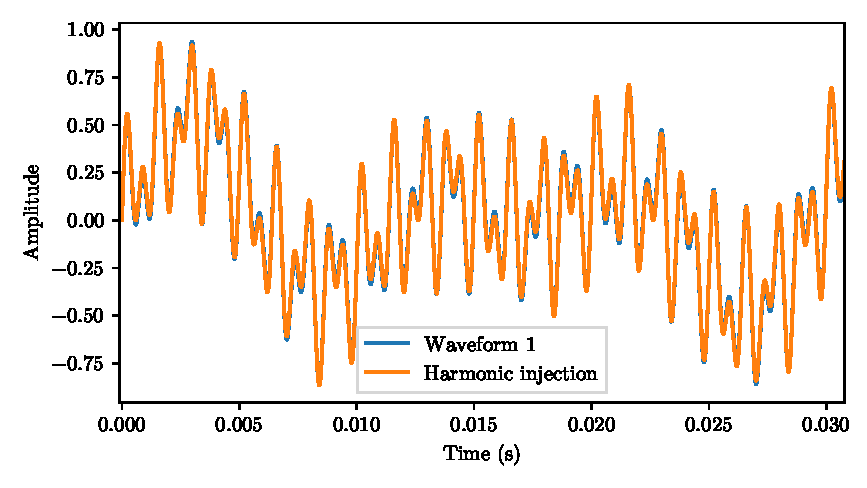
\includegraphics{Images/shaker/Figure_1.pdf}
    \caption{Waveform comparison of the shaker test.}
    \label{fig:shaker}
\end{figure}

\begin{figure}
    \centering
    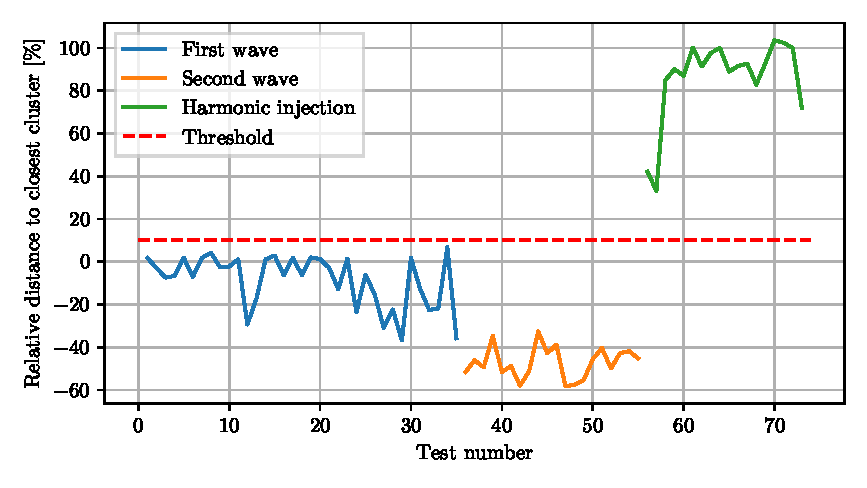
\includegraphics{Images/shaker/Results.pdf}
    \caption{Novelty detection result}
    \label{fig:shaker_results}
\end{figure}

\begin{figure}
    \centering
    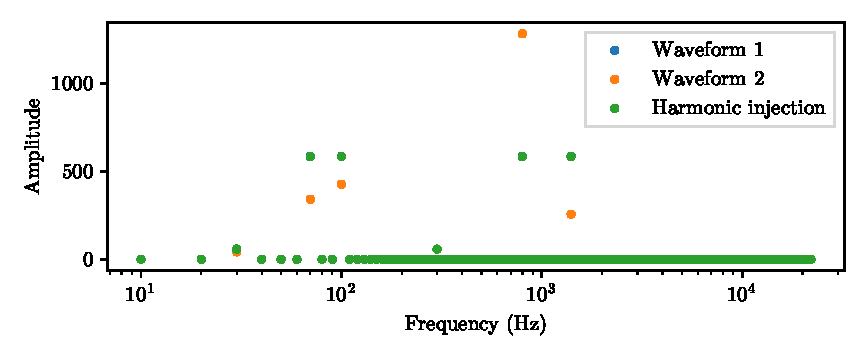
\includegraphics{Images/shaker/spectrum.pdf}
    \caption{Spectrum of the waveforms.}
    \label{fig:shaker_spectrum}
\end{figure}



\section{Experiments on a laboratory shaker - Test 2}
\label{sec:shaker_test02}
In the previous section, the first test on the shaker was presented. The test has shown the capability of the framework to detect unknown harmonics. A second test was done to evaluate the capability to detect time-domain variations and the effect of reducing the frequency resolution. 

\subsection{Training and evaluating}
This new configuration has been set to use only 4 frequency-domain features and the same 3 time-domain features of the previous test, for a total of 7 features. The signal used for training and testing is resumed in \autoref{tab:shaker_param_02}. The set is composed of the same signal at different amplitudes used for training and testing, plus another signal with different frequency content but the same amplitude as a training signal used for testing. 

The training has been carried out in the same way as the previous test, the training of the K-means model has been done with 4 \gls{glo:clust}s, and loaded on the microcontroller. 

\begin{table}
    \centering
    \caption{Parameters of the second shaker test.}
    \label{tab:shaker_param_02}
    \begin{tabular}{cccccccc} 
    \toprule
    \multicolumn{5}{c}{\textbf{Harmonic frequency} {[}Hz]} & \multirow{2}{*}{\textbf{Amplitude }{[}mV$_{pp}$]} & \multicolumn{2}{c}{\textbf{ No. of \gls{glo:snap}s}} \\
    10 & 30 & 60 & 70 & 100 &  & Train & Test \\ 
    \hline
    - & 0.1 & - & 1.0 & 1.0 & 580 & 100 & 10 \\
    - & 0.1 & - & 1.0 & 1.0 & 1000 & 100 & 10 \\
    - & 0.1 & - & 1.0 & 1.0 & 1980 & 100 & 10 \\
    - & 0.1 & - & 1.0 & 1.0 & 1540 & 100 & 10 \\
    - & 0.1 & - & 1.0 & 1.0 & 2000 & - & 20 \\
    - & 0.1 & - & 1.0 & 1.0 & 0 & - & 10 \\
    - & 0.1 & - & 1.0 & 1.0 & 800 & - & 10 \\
    - & 0.1 & - & 1.0 & 1.0 & 200 & - & 10 \\
    - & 0.1 & - & 1.0 & 1.0 & 1220 & - & 10 \\
    1.0 & 1.0 & 0.1 & - & - & 1540 & - & 10 \\
    \bottomrule
    \end{tabular}
    \end{table}



\subsection{Results}
\begin{figure}
    \centering
    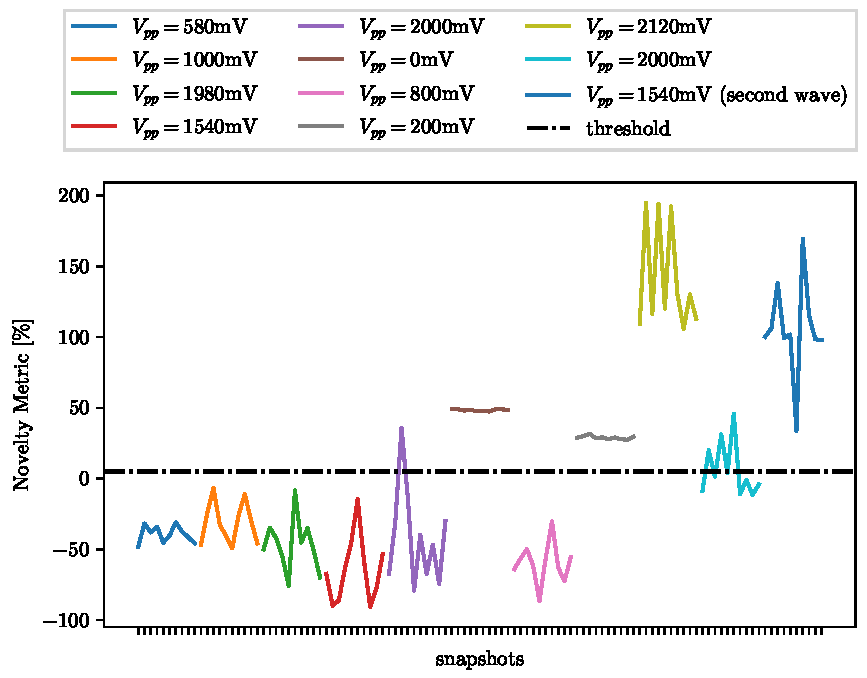
\includegraphics{Images/shaker/Test02.pdf}
    \caption{Novelty detection result}
    \label{fig:shaker_results02}
\end{figure}
The result of the novelty detection is shown in \autoref{fig:shaker_results02}. The first 4 lines have been correctly identified as normal, as they were in fact a repetition of the training signals.
Then the purple and cyan line in the figure is the same training signal, but 20 mV higher in amplitude \gls{wrt} the training signal. The novelty metric overshoots the threshold in 5 samples out of 20. An increase of 2\% in amplitude generates the \gls{nd} event 25\% of the times can be observed with this signal. 

The brown, grey and light-green lines are the same signal, but with a bigger difference in amplitude \gls{wrt} the training signal. All the \gls{glo:snap}s of these signals correctly generated a novelty metric above the threshold. The blue line is the signal with a different frequency content, and it has been correctly identified as a novelty event, this is the confirmation that even with just 4 frequency bins, the wavelet decomposition is still generating features that are informative.

The pink line is the test signal with an amplitude of 800mV. It's evident that the novelty metric is below the threshold, and the signal has been classified as normal even if it is not in the training dataset. Let's investigate how this happened. The first consideration is that the 800mV amplitude is quite tight to both the 1000mV and 580mV signals used for training. Moreover, in this case, the total number of features is just 7. This allows plotting all the features against each other, to see why the \gls{nd} event has not been detected. In \autoref{fig:shaker_conf_matrix} the scatter plot of the features is shown. It's evident that, in this environment, even performing the standardization of the features, the \gls{glo:clust}s are still very elongated, resembling almost a line. To fit an elongated \gls{glo:clust} in a hypersphere, it is inevitable that in some sections, the hypersphere will not closely surround the \gls{glo:clust}, leaving \quoted{space} for false negative results. Another problem is that the k-means algorithm tends to split long \gls{glo:clust}s. In the figure, the red dots are the false negative results, and the grey shades are the hypersphere projection on the considered features plane. The black dots are the training data. The effect of the elongated \gls{glo:clust}s is particularly evident in the plot of the \quoted{Feature 3} against \quoted{Feature 2}, where the red dots are in between two \gls{glo:clust}s, that are modelled as one. On the other hand, looking at the plot of \quoted{Feature 1} against \quoted{Feature 4}, a very long \gls{glo:clust} has been split in two. This is an example of exploiting the limitations of the k-means algorithm anticipated in \autoref{sec:kmeans_limits}. 
For completness, in \autoref{fig:shaker_conf_matrix}, also the true positive results are shown, as magenta dots.


\begin{figure}
    \centering
    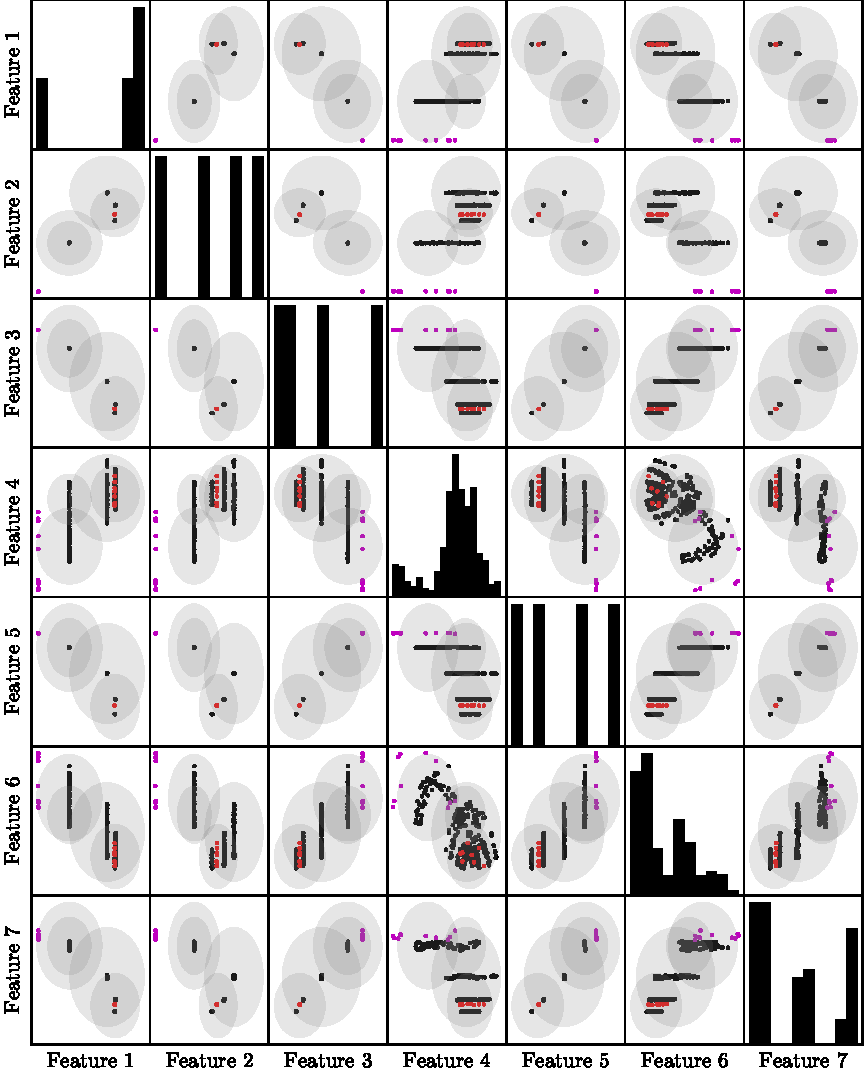
\includegraphics{Images/shaker/ConfusionMatrix.pdf}
    \caption{False Negative and True Positive results. On the diagonal, there is a histogram of the feature values. The off-diagonal plots are the scatter plots of the features. The shades are the projection of the \gls{glo:clust}s on the considered plane. (Red: False Negative, Magenta: True Positive, Black: training data)}
    \label{fig:shaker_conf_matrix}
\end{figure}
\clearpage

\subsection{Possible improvements}
The environment of this test is very challenging for the k-means algorithm. As discussed in \autoref{ch:Unsupervised}, there are algorithms that are not affected by the \gls{glo:clust}s' shapes. The candidate algorithms that may perform better in this situation are the \gls{lof}, the \gls{iforest} and \gls{dbscan}. Future work could be to implement these algorithms in the \gls{glo:edge} framework, despite being more demanding in computational power and memory, and test them in this environment.

As proof of concept, the \gls{lof} implementation in \texttt{\gls{glo:python}} has been used to perform \gls{nd} on the same dataset used in this section in \gls{glo:edge}. The results are reported in \autoref{label:lof_results}. The \gls{lof} algorithm has been able to correctly identify all the \gls{nd} events, even the signals with just 20mV variation from the training dataset, and the 800mV signal that was problematic for the K-means. The \gls{lof}, however, generated a false positive on the 580mV signal. This false positive may be avoided by increasing the threshold, but this would also increase the false negative rate. 

\begin{figure}
    \centering
    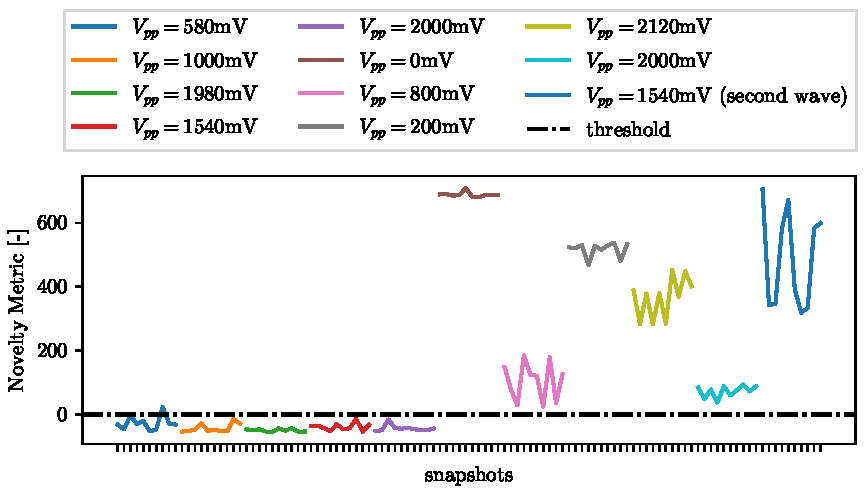
\includegraphics{Images/shaker/Test02_LOF.pdf}
    \caption{\gls{lof} novelty detection result}
    \label{fig:lof_results}
\end{figure}
\section{Experimental validation}
\label{sec:ExperimentalValidation}
